\begin{figure*}[!t]
	\begin{center}
		\subfloat[]{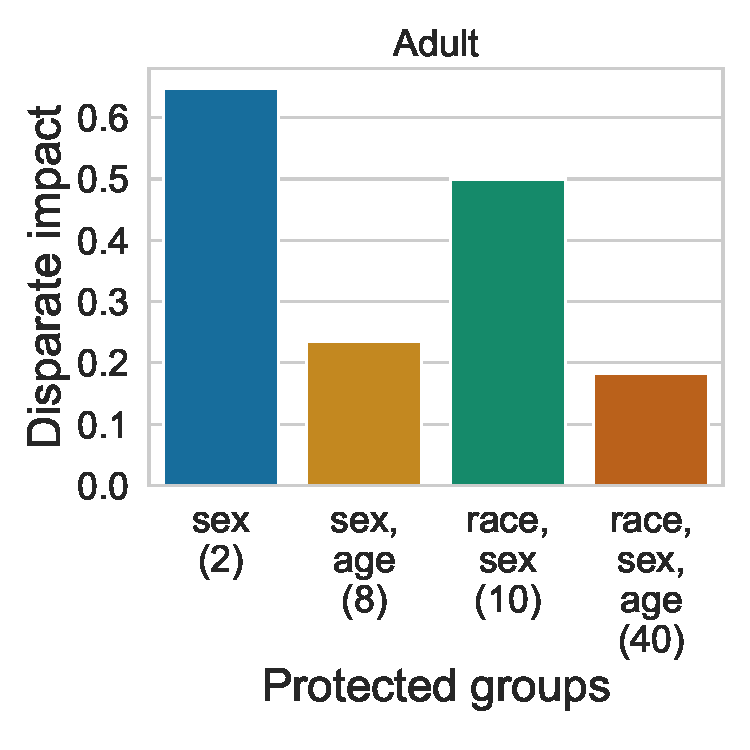
\includegraphics[scale=0.33]{figures/sensitive_attribute__Disparate_impact_Adult_LR_Learn-efficient-dependency}}
		\subfloat[]{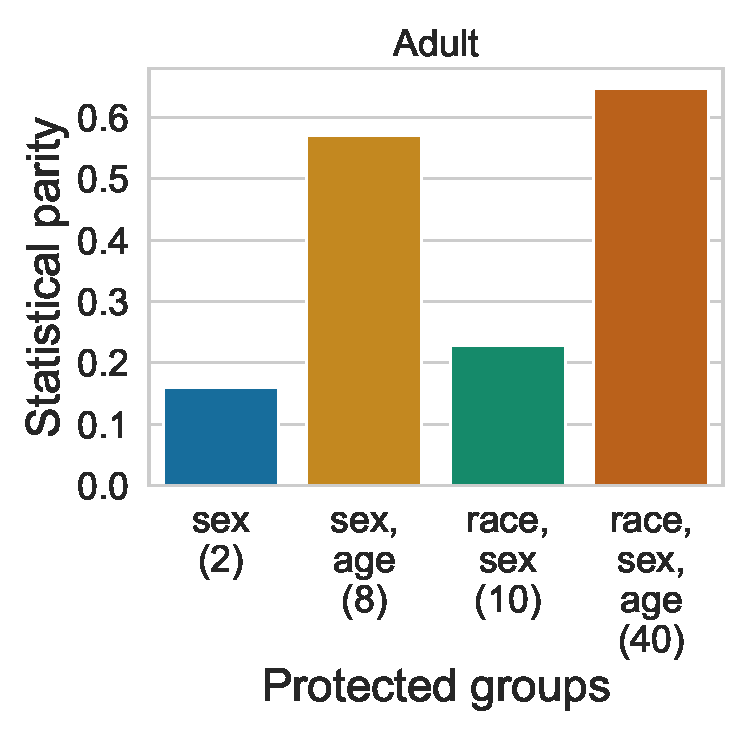
\includegraphics[scale=0.33]{figures/sensitive_attribute__Statistical_parity_Adult_LR_Learn-efficient-dependency}}
		\subfloat[]{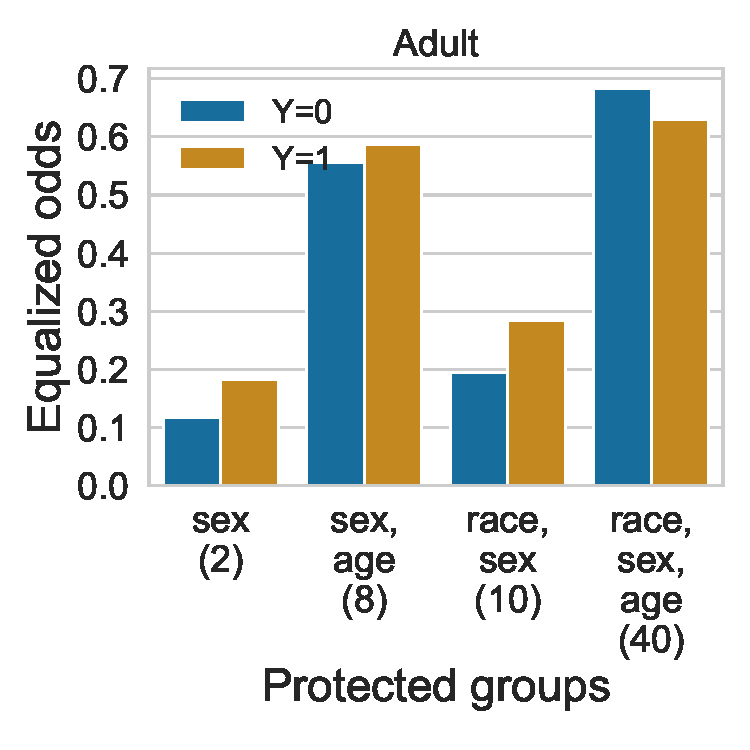
\includegraphics[scale=0.33]{figures/sensitive_attribute_eqo_Adult_LR_Learn-efficient-dependency}}
		\subfloat[]{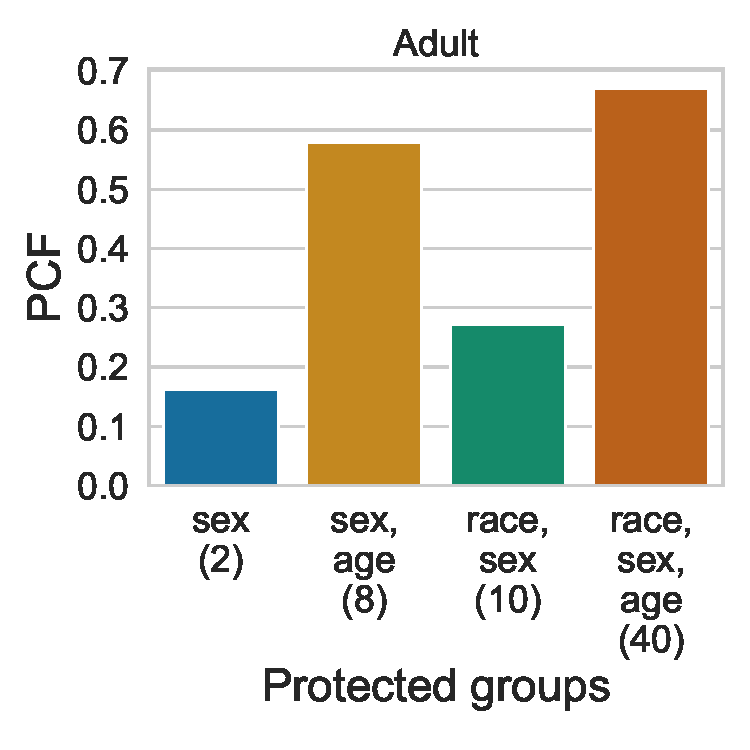
\includegraphics[scale=0.33]{figures/sensitive_attribute__PCF_Adult_LR_Learn-efficient-dependency}}	
		\\
		
		\subfloat[]{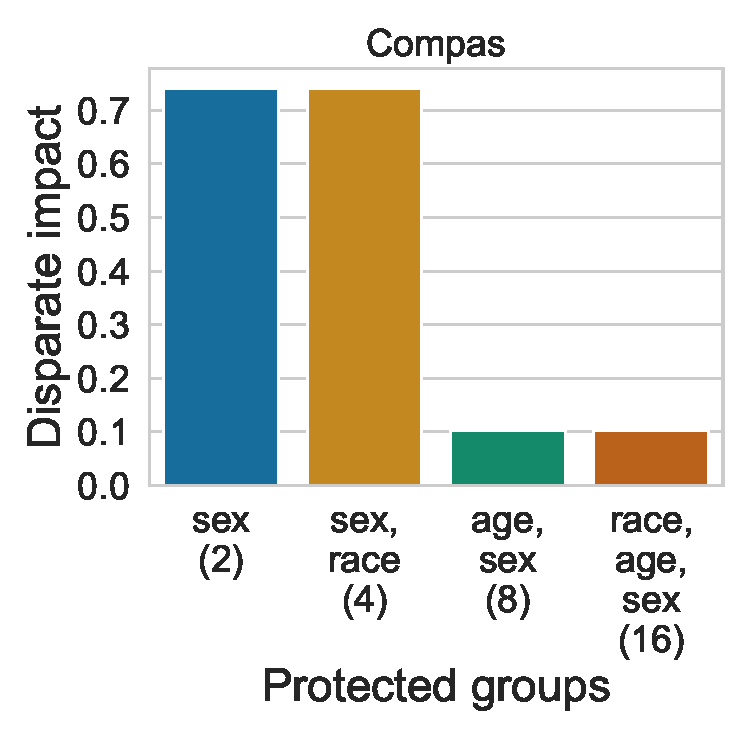
\includegraphics[scale=0.33]{figures/sensitive_attribute__Disparate_impact_Compas_LR_Learn-efficient-dependency}}			
		\subfloat[]{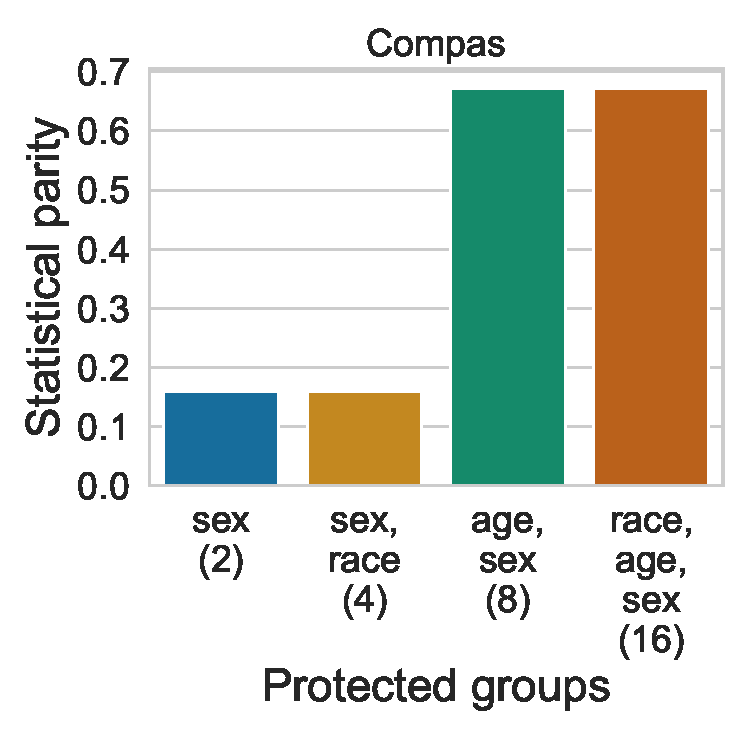
\includegraphics[scale=0.33]{figures/sensitive_attribute__Statistical_parity_Compas_LR_Learn-efficient-dependency}}
		\subfloat[]{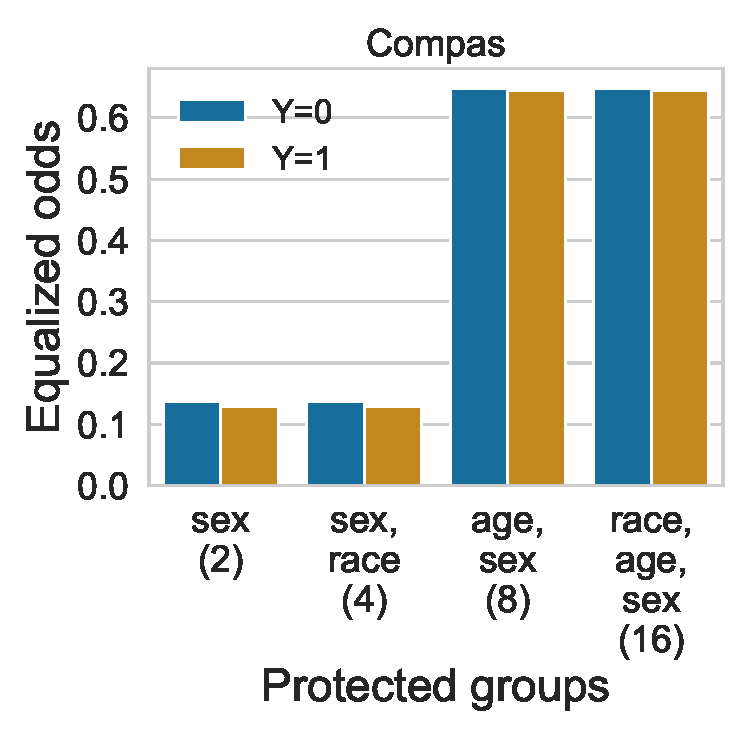
\includegraphics[scale=0.33]{figures/sensitive_attribute_eqo_Compas_LR_Learn-efficient-dependency}}
		\subfloat[]{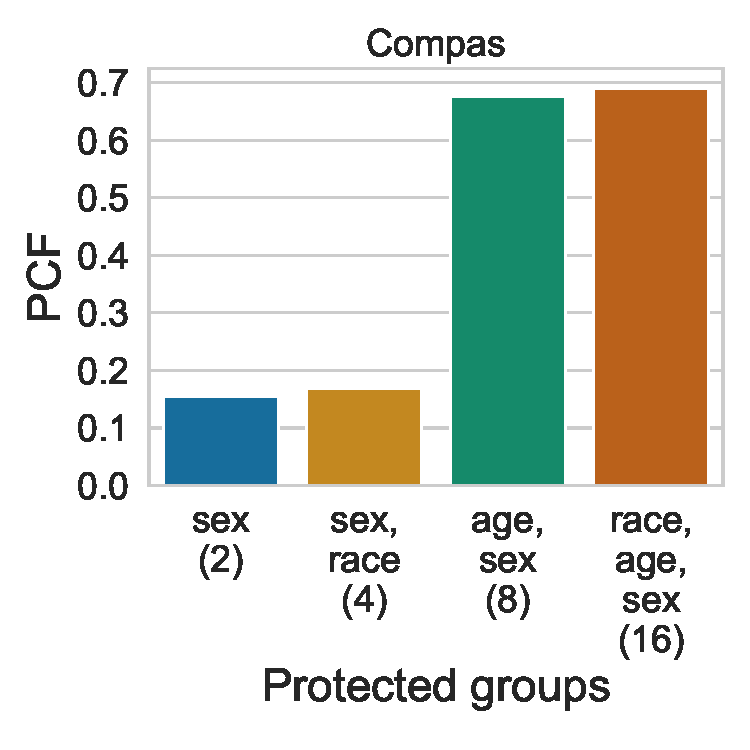
\includegraphics[scale=0.33]{figures/sensitive_attribute__PCF_Compas_LR_Learn-efficient-dependency}}	
		
	\end{center}
		\caption{Verifying compound sensitive groups with respect to multiple fairness metrics. In each plot, the $ X $-axis shows sensitive features with the number of compound groups (within parenthesis) and $ Y $-axis shows computed group and causal fairness metrics. }
		\label{fig:multiple_metrics}

\end{figure*}
	
	
	
